\documentclass[]{article}
\usepackage[a4paper, total={15cm,25cm}]{geometry}% Was 23, but lengthened to 25 to get diagram on single page in Assignment mode.
\usepackage{fancyhdr}
\usepackage{graphicx}
\usepackage{amsmath}
\usepackage{amssymb}
\usepackage{xcolor}
\usepackage{tikz}
\usepackage{verbatim}
\usepackage{tcolorbox}
\usepackage{textcomp}
\usepackage{xcomment}
%opening
\title{PH 223 Week 6}
\author{Benjamin Bauml}
\date{Winter 2024}
\pagestyle{fancy}
\rhead{PH 223}
\chead{Winter 2024}
\lhead{Week 6}

% For Assignment, leave Purpose as 0. For Worksheet, set to 1. For Student Solution, set to 2. For Teacher Solution, set to 3.
\newcommand{\Purpose}{0}

\newcommand{\Exclusion}{0}
\newcommand{\PageTurn}{0}
\newcommand{\GrayProb}{0}
\newcommand{\Tipsy}{0}

% Assignment
\if\Purpose0
\renewcommand{\Exclusion}{1}
\fi
% Worksheet
\if\Purpose1
\renewcommand{\Exclusion}{1}
\renewcommand{\PageTurn}{1}
\fi
% Student Solution
\if\Purpose2
\renewcommand{\PageTurn}{1}
\renewcommand{\GrayProb}{1}
\fi
% Teaching Copy
\if\Purpose3
\renewcommand{\PageTurn}{1}
\renewcommand{\GrayProb}{1}
\renewcommand{\Tipsy}{1}
\fi

\if\Exclusion1
\xcomment{Title,Problem,ProblemSub,PassFig}
\fi

\def \NewQ {0}
\newcommand{\MaybePage}{
	\if\NewQ0
	\gdef \NewQ {\PageTurn}
	\else
	\newpage
	\fi
}

\newenvironment{Problem}[1]{
\MaybePage
\section*{#1}
\if\GrayProb1
\begin{tcolorbox}[colback=lightgray,colframe=lightgray,sharp corners,boxsep=1pt,left=0pt,right=0pt,top=0pt,bottom=0pt,after skip=2pt]
\else
\begin{tcolorbox}[colback=white,colframe=white,sharp corners,boxsep=1pt,left=0pt,right=0pt,top=0pt,bottom=0pt,after skip=2pt]
\fi
}{
\end{tcolorbox}\noindent
}

\newenvironment{ProblemSub}{
\if\GrayProb1
\begin{tcolorbox}[colback=lightgray,colframe=lightgray,sharp corners,boxsep=1pt,left=0pt,right=0pt,top=0pt,bottom=0pt,after skip=2pt]
\else
\begin{tcolorbox}[colback=white,colframe=white,sharp corners,boxsep=1pt,left=0pt,right=0pt,top=0pt,bottom=0pt,after skip=2pt]
\fi
}{
\end{tcolorbox}\noindent
}

\newenvironment{PassFig}{\begin{figure}[h]}{\end{figure}}

\newcommand{\TeachingTips}[1]{
\if\Tipsy1
\begin{tcolorbox}[colback=lightgray,colframe=black]
#1
\end{tcolorbox}
\fi
}

\newenvironment{Title}{\maketitle}{}

\newcommand{\Ohm}{\textohm{} }

\begin{document}
\begin{Title}
\begin{center}
	The first two problems are adapted from Grant Sherer. The final problem is adapted from Chapter 28 of the \textit{Student Workbook} for \textit{Physics for Scientists and Engineers}.
\end{center}
\end{Title}

\begin{Problem}{Activity 1}
	Three 45 \Ohm resistors are in parallel, connected to a 21 \Ohm resistor in series with a battery of potential difference 9 V.
\end{Problem}
\begin{ProblemSub}
	(a) Draw a diagram of the circuit and a voltage diagram for at least one loop.
\end{ProblemSub}
\begin{center}
	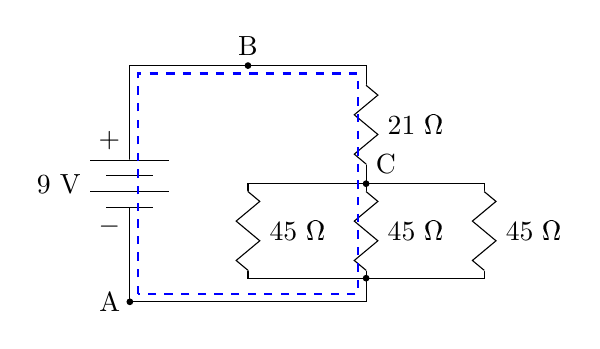
\begin{tikzpicture}
		\draw (0,0) -- (0,3) -- (3,3) -- (3,0) -- cycle;
		\draw (1.5,0.3) -- (1.5,1.5) -- (4.5,1.5) -- (4.5,0.3) -- cycle;
		\filldraw[black] (3,1.5) circle (1pt);
		\node[anchor=south west] at (3,1.5) {C};
		\filldraw[black] (3,0.3) circle (1pt);
		\filldraw[black] (0,0) circle (1pt);
		\node[anchor=east] at (0,0) {A};
		\filldraw[black] (1.5,3) circle (1pt);
		\node[anchor=south] at (1.5,3) {B};
		\begin{scope}[shift={(0,1.5)},rotate=-90]
			\filldraw[white] (-0.3,-0.5) -- (-0.3,0.5) -- (0.1,0.5) -- (0.3,0.3) -- (0.3,-0.3) -- (0.1,-0.5) -- (-0.3,-0.5) -- cycle;
			\draw (-0.3,-0.5) -- (-0.3,0.5);
			\draw (-0.1,-0.3) -- (-0.1,0.3);
			\draw (0.1,-0.5) -- (0.1,0.5);
			\draw (0.3,-0.3) -- (0.3,0.3);
		\end{scope}
		\node[anchor=north east] at (0,1.2) {$-$};
		\node[anchor=south east] at (0,1.8) {$+$};
		\node[anchor=east] at (-0.5,1.5) {9 V};
		\begin{scope}[shift={(3,2.25)},rotate=90]
			\filldraw[white] (0.5,0) -- (0.375,-0.15) -- (-0.125,-0.15) -- (-0.5,0) -- (-0.375,0.15) -- (0.125,0.15) -- cycle;
			\draw (0.5,0) -- (0.375,-0.15) -- (0.125,0.15) -- (-0.125,-0.15) -- (-0.375,0.15) -- (-0.5,0);
		\end{scope}
		\node[anchor=west] at (3.15,2.25) {21 \Ohm};
		\begin{scope}[shift={(1.5,0.9)},rotate=90]
			\filldraw[white] (0.5,0) -- (0.375,-0.15) -- (-0.125,-0.15) -- (-0.5,0) -- (-0.375,0.15) -- (0.125,0.15) -- cycle;
			\draw (0.5,0) -- (0.375,-0.15) -- (0.125,0.15) -- (-0.125,-0.15) -- (-0.375,0.15) -- (-0.5,0);
		\end{scope}
		\node[anchor=west] at (1.65,0.9) {45 \Ohm};
		\begin{scope}[shift={(3,0.9)},rotate=90]
			\filldraw[white] (0.5,0) -- (0.375,-0.15) -- (-0.125,-0.15) -- (-0.5,0) -- (-0.375,0.15) -- (0.125,0.15) -- cycle;
			\draw (0.5,0) -- (0.375,-0.15) -- (0.125,0.15) -- (-0.125,-0.15) -- (-0.375,0.15) -- (-0.5,0);
		\end{scope}
		\node[anchor=west] at (3.15,0.9) {45 \Ohm};
		\begin{scope}[shift={(4.5,0.9)},rotate=90]
			\filldraw[white] (0.5,0) -- (0.375,-0.15) -- (-0.125,-0.15) -- (-0.5,0) -- (-0.375,0.15) -- (0.125,0.15) -- cycle;
			\draw (0.5,0) -- (0.375,-0.15) -- (0.125,0.15) -- (-0.125,-0.15) -- (-0.375,0.15) -- (-0.5,0);
		\end{scope}
		\node[anchor=west] at (4.65,0.9) {45 \Ohm};
		\draw[dashed,blue,thick] (0.1,0.1) -- (0.1,2.9) -- (2.9,2.9) -- (2.9,0.1) -- cycle;
	\end{tikzpicture}
	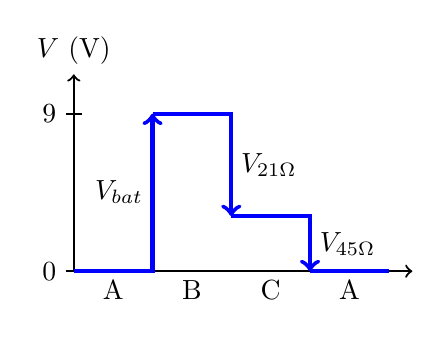
\begin{tikzpicture}
		\draw[->,thick] (0,0) -- (0,2.5);
		\node[anchor=south] at (0,2.5) {$V$ (V)};
		\draw[thick] (-0.1,2) -- (0.1,2);
		\node[anchor=east] at (-0.1,2) {9};
		\draw[->,thick] (-0.1,0) -- (4.3,0);
		\node[anchor=east] at (-0.1,0) {0};
		\draw[->,ultra thick,blue] (0,0) -- (1,0) -- (1,2);
		\node[anchor=east] at (1,1) {$V_{bat}$};
		\node[anchor=north] at (0.5,0) {A};
		\draw[->,ultra thick,blue] (1,2) -- (2,2) -- (2,0.7);
		\node[anchor=west] at (2,1.35) {$V_{21\Omega}$};
		\node[anchor=north] at (1.5,0) {B};
		\draw[->,ultra thick,blue] (2,0.7) -- (3,0.7) -- (3,0);
		\node[anchor=west] at (3,0.35) {$V_{45\Omega}$};
		\node[anchor=north] at (2.5,0) {C};
		\draw[ultra thick,blue] (3,0) -- (4,0);
		\node[anchor=north] at (3.5,0) {A};
	\end{tikzpicture}
	\begin{comment}
	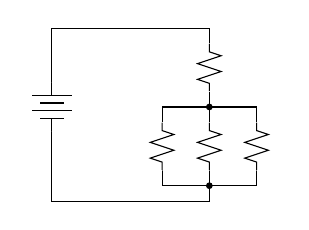
\begin{tikzpicture}
		\draw (0,0) -- (0,1) -- (2,1) -- (2,-1.2) -- (0,-1.2) -- cycle;
		\draw (1.4,0) -- (2.6,0) -- (2.6,-1) -- (1.4,-1) -- cycle;
		\filldraw[black] (2,0) circle (1pt);
		\filldraw[black] (2,-1) circle (1pt);
		\begin{scope}[shift={(0,0)},rotate=0]
			\filldraw[white] (0,0) circle (0.3);
			\draw (0,0.15) -- (0,0.3);
			\draw (-0.25,0.15) -- (0.25,0.15);
			\draw (-0.15,0.05) -- (0.15,0.05);
			\draw (-0.25,-0.05) -- (0.25,-0.05);
			\draw (-0.15,-0.15) -- (0.15,-0.15);
			\draw (0,-0.15) -- (0,-0.3);
		\end{scope}
		\begin{scope}[shift={(2,0.5)},rotate=0]
			\filldraw[white] (0,0) circle (0.3);
			\draw (0,0.3) -- (0,0.2) -- (0.15,0.15) -- (-0.15,0.05) -- (0.15,-0.05) -- (-0.15,-0.15) -- (0,-0.2) -- (0,-0.3);
		\end{scope}
		\begin{scope}[shift={(1.4,-0.5)},rotate=0]
		\filldraw[white] (0,0) circle (0.3);
		\draw (0,0.3) -- (0,0.2) -- (0.15,0.15) -- (-0.15,0.05) -- (0.15,-0.05) -- (-0.15,-0.15) -- (0,-0.2) -- (0,-0.3);
		\end{scope}
		\begin{scope}[shift={(2,-0.5)},rotate=0]
			\filldraw[white] (0,0) circle (0.3);
			\draw (0,0.3) -- (0,0.2) -- (0.15,0.15) -- (-0.15,0.05) -- (0.15,-0.05) -- (-0.15,-0.15) -- (0,-0.2) -- (0,-0.3);
		\end{scope}
		\begin{scope}[shift={(2.6,-0.5)},rotate=0]
		\filldraw[white] (0,0) circle (0.3);
		\draw (0,0.3) -- (0,0.2) -- (0.15,0.15) -- (-0.15,0.05) -- (0.15,-0.05) -- (-0.15,-0.15) -- (0,-0.2) -- (0,-0.3);
		\end{scope}
	\end{tikzpicture}
	\end{comment}
\end{center}
The voltage diagram depicts the voltage around the loop indicated in the circuit diagram by the dashed blue line. This diagram would have been valid through any of the three 45 \Ohm resistors. I have predicted that the voltage drop across the 21 \Ohm resistor will be larger, as there will be one third of the total current through each 45 \Ohm resistor:
\[
|V_{21\Omega}| = I(21\ \Omega) > I(15\ \Omega) = \frac{I}{3} (45\ \Omega) = |V_{45\Omega}|.
\]
\begin{ProblemSub}
	(b) Write loop and junction rules that completely characterize the circuit. (Use each resistor in at least 1 loop rule and 1 junction rule.)
\end{ProblemSub}
\begin{center}
	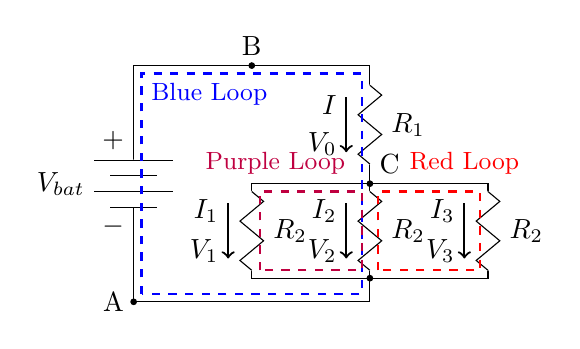
\begin{tikzpicture}
		\draw (0,0) -- (0,3) -- (3,3) -- (3,0) -- cycle;
		\draw (1.5,0.3) -- (1.5,1.5) -- (4.5,1.5) -- (4.5,0.3) -- cycle;
		\filldraw[black] (3,1.5) circle (1pt);
		\node[anchor=south west] at (3,1.5) {C};
		\filldraw[black] (3,0.3) circle (1pt);
		\filldraw[black] (0,0) circle (1pt);
		\node[anchor=east] at (0,0) {A};
		\filldraw[black] (1.5,3) circle (1pt);
		\node[anchor=south] at (1.5,3) {B};
		\begin{scope}[shift={(0,1.5)},rotate=-90]
			\filldraw[white] (-0.3,-0.5) -- (-0.3,0.5) -- (0.1,0.5) -- (0.3,0.3) -- (0.3,-0.3) -- (0.1,-0.5) -- (-0.3,-0.5) -- cycle;
			\draw (-0.3,-0.5) -- (-0.3,0.5);
			\draw (-0.1,-0.3) -- (-0.1,0.3);
			\draw (0.1,-0.5) -- (0.1,0.5);
			\draw (0.3,-0.3) -- (0.3,0.3);
		\end{scope}
		\node[anchor=north east] at (0,1.2) {$-$};
		\node[anchor=south east] at (0,1.8) {$+$};
		\node[anchor=east] at (-0.5,1.5) {$V_{bat}$};
		\begin{scope}[shift={(3,2.25)},rotate=90]
			\filldraw[white] (0.5,0) -- (0.375,-0.15) -- (-0.125,-0.15) -- (-0.5,0) -- (-0.375,0.15) -- (0.125,0.15) -- cycle;
			\draw (0.5,0) -- (0.375,-0.15) -- (0.125,0.15) -- (-0.125,-0.15) -- (-0.375,0.15) -- (-0.5,0);
		\end{scope}
		\node[anchor=west] at (3.15,2.25) {$R_{1}$};
		\draw[->,thick] (2.7,2.6) -- (2.7,1.9);
		\node[anchor=east] at (2.7,2.5) {$I$};
		\node[anchor=east] at (2.7,2) {$V_{0}$};
		\begin{scope}[shift={(1.5,0.9)},rotate=90]
			\filldraw[white] (0.5,0) -- (0.375,-0.15) -- (-0.125,-0.15) -- (-0.5,0) -- (-0.375,0.15) -- (0.125,0.15) -- cycle;
			\draw (0.5,0) -- (0.375,-0.15) -- (0.125,0.15) -- (-0.125,-0.15) -- (-0.375,0.15) -- (-0.5,0);
		\end{scope}
		\node[anchor=west] at (1.65,0.9) {$R_{2}$};
		\draw[->,thick] (1.2,1.25) -- (1.2,0.55);
		\node[anchor=east] at (1.2,1.15) {$I_{1}$};
		\node[anchor=east] at (1.2,0.65) {$V_{1}$};
		\begin{scope}[shift={(3,0.9)},rotate=90]
			\filldraw[white] (0.5,0) -- (0.375,-0.15) -- (-0.125,-0.15) -- (-0.5,0) -- (-0.375,0.15) -- (0.125,0.15) -- cycle;
			\draw (0.5,0) -- (0.375,-0.15) -- (0.125,0.15) -- (-0.125,-0.15) -- (-0.375,0.15) -- (-0.5,0);
		\end{scope}
		\node[anchor=west] at (3.15,0.9) {$R_{2}$};
		\begin{scope}[shift={(1.5,0)}]
			\draw[->,thick] (1.2,1.25) -- (1.2,0.55);
			\node[anchor=east] at (1.2,1.15) {$I_{2}$};
			\node[anchor=east] at (1.2,0.65) {$V_{2}$};
		\end{scope}
		\begin{scope}[shift={(4.5,0.9)},rotate=90]
			\filldraw[white] (0.5,0) -- (0.375,-0.15) -- (-0.125,-0.15) -- (-0.5,0) -- (-0.375,0.15) -- (0.125,0.15) -- cycle;
			\draw (0.5,0) -- (0.375,-0.15) -- (0.125,0.15) -- (-0.125,-0.15) -- (-0.375,0.15) -- (-0.5,0);
		\end{scope}
		\node[anchor=west] at (4.65,0.9) {$R_{2}$};
		\begin{scope}[shift={(3,0)}]
			\draw[->,thick] (1.2,1.25) -- (1.2,0.55);
			\node[anchor=east] at (1.2,1.15) {$I_{3}$};
			\node[anchor=east] at (1.2,0.65) {$V_{3}$};
		\end{scope}
		\draw[dashed,blue,thick] (0.1,0.1) -- (0.1,2.9) -- (2.9,2.9) -- (2.9,0.1) -- cycle;
		\node[anchor=north west] at (0.1,2.9) {\small\color{blue} Blue Loop};
		\draw[dashed,purple,thick] (1.6,0.4) -- (1.6,1.4) -- (2.9,1.4) -- (2.9,0.4) -- cycle;
		\node[anchor=south] at (1.8,1.5) {\small\color{purple} Purple Loop};
		\draw[dashed,red,thick] (3.1,0.4) -- (3.1,1.4) -- (4.4,1.4) -- (4.4,0.4) -- cycle;
		\node[anchor=south] at (4.2,1.5) {\small\color{red} Red Loop};
	\end{tikzpicture}
\end{center}
On the above picture, I have replaced each number from our original circuit diagram with a symbolic quantity, where $V_{bat} = 9$ V, $R_{1} = 21$ \Ohm and $R_{2} = 45\ \Omega$. The total current from the battery (and thus the current through the solitary $R_{1}$) is $I$, and the voltage drop across the $R_{1}$ resistor is $V_{0}$. The three $R_{2}$ resistors have been given their own currents and voltage drops (we know these should be identical between these resistors, but we will leave this in more generality for now as we set up the loop rules), ordered from left to right. Note that $V_{0},\ V_{1},\ V_{2}$, and $V_{3}$ are negative quantities, as they are describing the change in voltage across the resistors when following the current flow.

I have also explicitly marked three loops. The blue loop goes through the battery, through $R_{1}$, and finally through the middle $R_{2}$. The purple loop goes through the left and middle $R_{2}$ resistors, while the red loop goes through the center and right $R_{2}$ resistors. Let us traverse all of these loops clockwise, which will be important when introducing signs in our loop rules.

We have two junctions (one at C and one unmarked below it), but they are both characterized by the same junction rule:
\[
I = I_{1}+I_{2}+I_{3}.
\]
The blue loop is characterized by the following loop rule:
\[
V_{bat} + V_{0} + V_{2} = 0.
\]
The purple loop is characterized by
\[
-V_{1} + V_{2} = 0,
\]
where a negative sign has been added to $V_{1}$ since we are going against the flow of current (turning the negative quantity $V_{1}$ into a positive voltage change). Similarly, the red loop is characterized by
\[
-V_{2} + V_{3} = 0.
\]
\begin{ProblemSub}
	(c) Find $R_{eq}$.
\end{ProblemSub}
For the three resistors in parallel, we have
\[
\frac{1}{R_{eq,3}} = \frac{1}{R_{2}} + \frac{1}{R_{2}} + \frac{1}{R_{2}} = \frac{3}{R_{2}} \implies R_{eq,3} = \frac{R_{2}}{3}.
\]
This trio is in series with $R_{1}$, so they add directly to gain the overall equivalent resistance
\[
R_{eq} = R_{1} + R_{eq,3} = R_{1} + \frac{R_{2}}{3}.
\]
Plugging in our given numbers, we obtain $R_{eq} = 36\ \Omega$.

\begin{Problem}{Activity 2}
	Sketch a circuit that uses any number of 12 \Ohm resistors to create an equivalent resistance of:
\end{Problem}
\begin{ProblemSub}
	(a) 60 \Ohm
\end{ProblemSub}
To get a larger resistance, we know we will need to be adding resistors in series. In particular, five 12 \Ohm resistors in series have an equivalent resistance of 60 \Ohm.
\begin{center}
	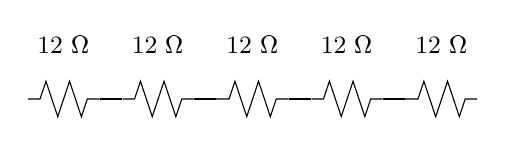
\begin{tikzpicture}[scale=1.5]
		\draw (0,0) -- (3.2,0);
		\begin{scope}[shift={(0,0)},rotate=90]
			\filldraw[white] (0,0) circle (0.3);
			\draw (0,0.3) -- (0,0.2) -- (0.15,0.15) -- (-0.15,0.05) -- (0.15,-0.05) -- (-0.15,-0.15) -- (0,-0.2) -- (0,-0.3);
		\end{scope}
		\node[anchor=south] at (0,0.3) {\small 12 \Ohm};
		\begin{scope}[shift={(0.8,0)},rotate=90]
			\filldraw[white] (0,0) circle (0.3);
			\draw (0,0.3) -- (0,0.2) -- (0.15,0.15) -- (-0.15,0.05) -- (0.15,-0.05) -- (-0.15,-0.15) -- (0,-0.2) -- (0,-0.3);
		\end{scope}
		\node[anchor=south] at (0.8,0.3) {\small 12 \Ohm};
		\begin{scope}[shift={(1.6,0)},rotate=90]
			\filldraw[white] (0,0) circle (0.3);
			\draw (0,0.3) -- (0,0.2) -- (0.15,0.15) -- (-0.15,0.05) -- (0.15,-0.05) -- (-0.15,-0.15) -- (0,-0.2) -- (0,-0.3);
		\end{scope}
		\node[anchor=south] at (1.6,0.3) {\small 12 \Ohm};
		\begin{scope}[shift={(2.4,0)},rotate=90]
			\filldraw[white] (0,0) circle (0.3);
			\draw (0,0.3) -- (0,0.2) -- (0.15,0.15) -- (-0.15,0.05) -- (0.15,-0.05) -- (-0.15,-0.15) -- (0,-0.2) -- (0,-0.3);
		\end{scope}
		\node[anchor=south] at (2.4,0.3) {\small 12 \Ohm};
		\begin{scope}[shift={(3.2,0)},rotate=90]
			\filldraw[white] (0,0) circle (0.3);
			\draw (0,0.3) -- (0,0.2) -- (0.15,0.15) -- (-0.15,0.05) -- (0.15,-0.05) -- (-0.15,-0.15) -- (0,-0.2) -- (0,-0.3);
		\end{scope}
		\node[anchor=south] at (3.2,0.3) {\small 12 \Ohm};
	\end{tikzpicture}
\end{center}
\begin{ProblemSub}
	(b) 3 \Ohm
\end{ProblemSub}
To get a smaller resistance, we know we will need to be adding resistors in parallel. In general, the equivalent resistance $R_{eq}$ of adding $n$ resistors (the $i$th resistor having resistance $R_{i}$) in parallel is given by
\[
\frac{1}{R_{eq}} = \frac{1}{R_{1}} + \frac{1}{R_{2}} + \frac{1}{R_{3}} + \dots + \frac{1}{R_{n}}.
\]
If the resistors are identical ($R_{i} = R$ for all $i$), then this simplifies to
\[
\frac{1}{R_{eq}} = \frac{n}{R},
\]
which means $R_{eq} = \frac{R}{n}$ for $n$ identical resistors in parallel.

In this particular case, 3 is equal to 12 divided by 4, so we can achieve an equivalent resistance of 3 \Ohm by putting four 12 \Ohm resistors in parallel.
\begin{center}
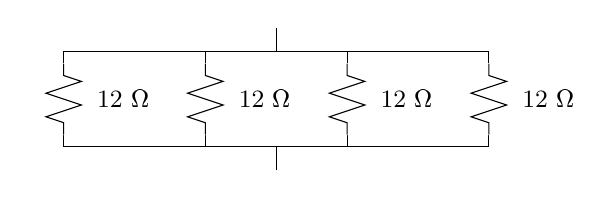
\begin{tikzpicture}[scale=1.5]
	\draw (1.8,0.6) -- (1.8,0.4) -- (3.6,0.4) -- (3.6,-0.4) -- (1.8,-0.4) -- (1.8,-0.6);
	\draw (1.8,0.6) -- (1.8,0.4) -- (0,0.4) -- (0,-0.4) -- (1.8,-0.4) -- (1.8,-0.6);
	\draw (1.2,0.4) -- (1.2,-0.4);
	\draw (2.4,0.4) -- (2.4,-0.4);
	\begin{scope}[shift={(0,0)},rotate=0]
		\filldraw[white] (0,0) circle (0.3);
		\draw (0,0.3) -- (0,0.2) -- (0.15,0.15) -- (-0.15,0.05) -- (0.15,-0.05) -- (-0.15,-0.15) -- (0,-0.2) -- (0,-0.3);
	\end{scope}
	\node[anchor=west] at (0.2,0) {\small 12 \Ohm};
	\begin{scope}[shift={(1.2,0)},rotate=0]
		\filldraw[white] (0,0) circle (0.3);
		\draw (0,0.3) -- (0,0.2) -- (0.15,0.15) -- (-0.15,0.05) -- (0.15,-0.05) -- (-0.15,-0.15) -- (0,-0.2) -- (0,-0.3);
	\end{scope}
	\node[anchor=west] at (1.4,0) {\small 12 \Ohm};
	\begin{scope}[shift={(2.4,0)},rotate=0]
		\filldraw[white] (0,0) circle (0.3);
		\draw (0,0.3) -- (0,0.2) -- (0.15,0.15) -- (-0.15,0.05) -- (0.15,-0.05) -- (-0.15,-0.15) -- (0,-0.2) -- (0,-0.3);
	\end{scope}
	\node[anchor=west] at (2.6,0) {\small 12 \Ohm};
	\begin{scope}[shift={(3.6,0)},rotate=0]
		\filldraw[white] (0,0) circle (0.3);
		\draw (0,0.3) -- (0,0.2) -- (0.15,0.15) -- (-0.15,0.05) -- (0.15,-0.05) -- (-0.15,-0.15) -- (0,-0.2) -- (0,-0.3);
	\end{scope}
	\node[anchor=west] at (3.8,0) {\small 12 \Ohm};
\end{tikzpicture}
\end{center}
\begin{ProblemSub}
	(c) 10 \Ohm
\end{ProblemSub}
This equivalent resistance is smaller, so we will need to use parallel resistors, but it isn't as simple as part (b), as there is no integer which divides 12 to give 10. Still, we can put a few identical ones in parallel to give ourselves some (resistance-wise) smaller building blocks to work with. Once we have these smaller equivalent resistors, we can try to put some of them in series to increase our total resistance back toward the goal.

In particular, note that two 12 \Ohm resistors in parallel have an equivalent resistance of 6 \Ohm, and three of these resistors in parallel have an equivalent resistance of 4 \Ohm. By putting the two parallel resistors in series with the three parallel resistors, we get an overall equivalent resistance of 10 \Ohm.
\begin{center}
	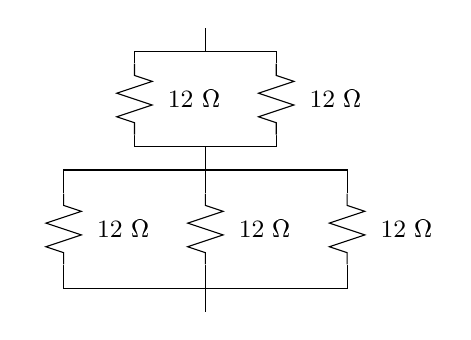
\begin{tikzpicture}[scale=1.5]
		\draw (0,0.6) -- (0,0.4);
		\draw (-0.6,0.4) -- (0.6,0.4) -- (0.6,-0.4) -- (-0.6,-0.4) -- cycle;
		\draw (0,-1.8) -- (0,-0.4);
		\draw (-1.2,-0.6) -- (1.2,-0.6) -- (1.2,-1.6) -- (-1.2,-1.6) -- cycle;
		\begin{scope}[shift={(-0.6,0)},rotate=0]
			\filldraw[white] (0,0) circle (0.3);
			\draw (0,0.3) -- (0,0.2) -- (0.15,0.15) -- (-0.15,0.05) -- (0.15,-0.05) -- (-0.15,-0.15) -- (0,-0.2) -- (0,-0.3);
		\end{scope}
		\node[anchor=west] at (-0.4,0) {\small 12 \Ohm};
		\begin{scope}[shift={(0.6,0)},rotate=0]
			\filldraw[white] (0,0) circle (0.3);
			\draw (0,0.3) -- (0,0.2) -- (0.15,0.15) -- (-0.15,0.05) -- (0.15,-0.05) -- (-0.15,-0.15) -- (0,-0.2) -- (0,-0.3);
		\end{scope}
		\node[anchor=west] at (0.8,0) {\small 12 \Ohm};
		\begin{scope}[shift={(-1.2,-1.1)},rotate=0]
			\filldraw[white] (0,0) circle (0.3);
			\draw (0,0.3) -- (0,0.2) -- (0.15,0.15) -- (-0.15,0.05) -- (0.15,-0.05) -- (-0.15,-0.15) -- (0,-0.2) -- (0,-0.3);
		\end{scope}
		\node[anchor=west] at (-1,-1.1) {\small 12 \Ohm};
		\begin{scope}[shift={(0,-1.1)},rotate=0]
			\filldraw[white] (0,0) circle (0.3);
			\draw (0,0.3) -- (0,0.2) -- (0.15,0.15) -- (-0.15,0.05) -- (0.15,-0.05) -- (-0.15,-0.15) -- (0,-0.2) -- (0,-0.3);
		\end{scope}
		\node[anchor=west] at (0.2,-1.1) {\small 12 \Ohm};
		\begin{scope}[shift={(1.2,-1.1)},rotate=0]
			\filldraw[white] (0,0) circle (0.3);
			\draw (0,0.3) -- (0,0.2) -- (0.15,0.15) -- (-0.15,0.05) -- (0.15,-0.05) -- (-0.15,-0.15) -- (0,-0.2) -- (0,-0.3);
		\end{scope}
		\node[anchor=west] at (1.4,-1.1) {\small 12 \Ohm};
	\end{tikzpicture}
\end{center}

\begin{Problem}{Activity 3}
	(a) Draw a circuit for which the Kirchhoff's loop law equation is
	\[
	6\text{ V} - I\cdot 2\text{ \Ohm} + 3\text{ V} - I\cdot4\text{ \Ohm} = 0.
	\]
	Assume that the analysis is done in a clockwise direction.
\end{Problem}
First, note that $ - I\cdot 2\text{ \Ohm} $ and $ - I\cdot4\text{ \Ohm} $ are voltage drops across resistors. The voltage change across a resistor is negative when we are tracing our loop in agreement with the direction of the current. As such, the current is flowing clockwise. The other two voltage differences appear to be gains from moving from the negative terminal of a battery to the positive terminal of a battery.
\begin{center}
	\begin{tikzpicture}
		\draw (0,0) -- (0,3) -- (3,3) -- (3,0) -- cycle;
		\begin{scope}[shift={(1.5,0)},rotate=0]
			\filldraw[white] (0.5,0) -- (0.375,-0.15) -- (-0.125,-0.15) -- (-0.5,0) -- (-0.375,0.15) -- (0.125,0.15) -- cycle;
			\draw (0.5,0) -- (0.375,-0.15) -- (0.125,0.15) -- (-0.125,-0.15) -- (-0.375,0.15) -- (-0.5,0);
		\end{scope}
		\node[anchor=north] at (1.5,-0.15) {4 \Ohm};
		\begin{scope}[shift={(1.5,3)},rotate=0]
			\filldraw[white] (0.5,0) -- (0.375,-0.15) -- (-0.125,-0.15) -- (-0.5,0) -- (-0.375,0.15) -- (0.125,0.15) -- cycle;
			\draw (0.5,0) -- (0.375,-0.15) -- (0.125,0.15) -- (-0.125,-0.15) -- (-0.375,0.15) -- (-0.5,0);
		\end{scope}
		\node[anchor=south] at (1.5,3.15) {2 \Ohm};
		\begin{scope}[shift={(0,1.5)},rotate=-90]
			\filldraw[white] (-0.3,-0.5) -- (-0.3,0.5) -- (0.1,0.5) -- (0.3,0.3) -- (0.3,-0.3) -- (0.1,-0.5) -- (-0.3,-0.5) -- cycle;
			\draw (-0.3,-0.5) -- (-0.3,0.5);
			\draw (-0.1,-0.3) -- (-0.1,0.3);
			\draw (0.1,-0.5) -- (0.1,0.5);
			\draw (0.3,-0.3) -- (0.3,0.3);
		\end{scope}
		\node[anchor=north east] at (0,1.2) {$-$};
		\node[anchor=south east] at (0,1.8) {$+$};
		\node[anchor=east] at (-0.5,1.5) {6 V};
		\begin{scope}[shift={(3,1.5)},rotate=90]
			\filldraw[white] (-0.3,-0.5) -- (-0.3,0.5) -- (0.1,0.5) -- (0.3,0.3) -- (0.3,-0.3) -- (0.1,-0.5) -- (-0.3,-0.5) -- cycle;
			\draw (-0.3,-0.5) -- (-0.3,0.5);
			\draw (-0.1,-0.3) -- (-0.1,0.3);
			\draw (0.1,-0.5) -- (0.1,0.5);
			\draw (0.3,-0.3) -- (0.3,0.3);
		\end{scope}
		\node[anchor=north west] at (3,1.2) {$+$};
		\node[anchor=south west] at (3,1.8) {$-$};
		\node[anchor=west] at (3.5,1.5) {3 V};
	\end{tikzpicture}
\end{center}
\begin{ProblemSub}
	(b) A voltage diagram is shown below for a different circuit. The current in the circuit is 2.0 A. Draw the circuit diagram and identify the points on the circuit diagram that are on the voltage diagram.
\end{ProblemSub}
\begin{PassFig}
	\centering
	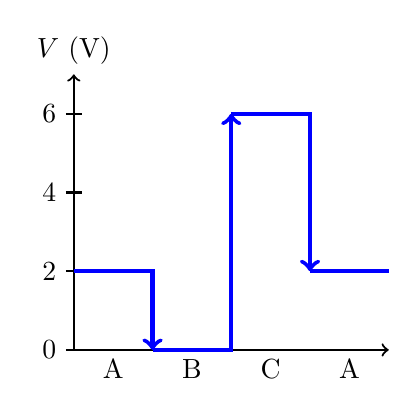
\begin{tikzpicture}
		\draw[->,thick] (0,0) -- (0,3.5);
		\node[anchor=south] at (0,3.5) {$V$ (V)};
		\draw[thick] (-0.1,1) -- (0.1,1);
		\node[anchor=east] at (-0.1,1) {2};
		\draw[thick] (-0.1,2) -- (0.1,2);
		\node[anchor=east] at (-0.1,2) {4};
		\draw[thick] (-0.1,3) -- (0.1,3);
		\node[anchor=east] at (-0.1,3) {6};
		\draw[->,thick] (-0.1,0) -- (4,0);
		\node[anchor=east] at (-0.1,0) {0};
		\draw[->,ultra thick,blue] (0,1) -- (1,1) -- (1,0);
		\node[anchor=north] at (0.5,0) {A};
		\draw[->,ultra thick,blue] (1,0) -- (2,0) -- (2,3);
		\node[anchor=north] at (1.5,0) {B};
		\draw[->,ultra thick,blue] (2,3) -- (3,3) -- (3,1);
		\node[anchor=north] at (2.5,0) {C};
		\draw[ultra thick,blue] (3,1) -- (4,1);
		\node[anchor=north] at (3.5,0) {A};
	\end{tikzpicture}
\end{PassFig}

Moving in agreement with the current, we see that the voltage goes down by 2 V when we cross the first circuit element (the horizontal regions in between the vertical arrows are wires acting as perfect conductors). A 1 \Ohm resistor would have this voltage drop for 2.0 A of current. The next circuit component increases the potential by six volts, which suggests that we have gone from the negative terminal to the positive terminal of a 6 V battery. Finally we drop 4 V in the last circuit element, and this can be accomplished by a 2 \Ohm resistor at 2.0 A.
\begin{center}
	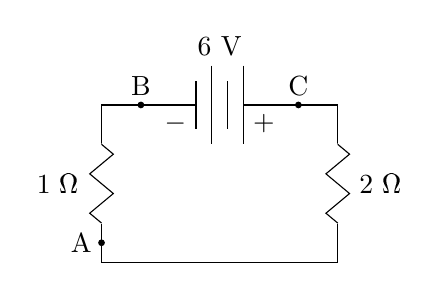
\begin{tikzpicture}
		\draw (0,0) -- (0,2) -- (3,2) -- (3,0) -- cycle;
		\filldraw[black] (0,0.25) circle (1pt);
		\node[anchor=east] at (0,0.25) {A};
		\begin{scope}[shift={(0,1)},rotate=90]
			\filldraw[white] (0.5,0) -- (0.375,-0.15) -- (-0.125,-0.15) -- (-0.5,0) -- (-0.375,0.15) -- (0.125,0.15) -- cycle;
			\draw (0.5,0) -- (0.375,-0.15) -- (0.125,0.15) -- (-0.125,-0.15) -- (-0.375,0.15) -- (-0.5,0);
		\end{scope}
		\node[anchor=east] at (-0.15,1) {1 \Ohm};
		\filldraw[black] (0.5,2) circle (1pt);
		\node[anchor=south] at (0.5,2) {B};
		\begin{scope}[shift={(1.5,2)},rotate=180]
			\filldraw[white] (-0.3,-0.5) -- (-0.3,0.5) -- (0.1,0.5) -- (0.3,0.3) -- (0.3,-0.3) -- (0.1,-0.5) -- (-0.3,-0.5) -- cycle;
			\draw (-0.3,-0.5) -- (-0.3,0.5);
			\draw (-0.1,-0.3) -- (-0.1,0.3);
			\draw (0.1,-0.5) -- (0.1,0.5);
			\draw (0.3,-0.3) -- (0.3,0.3);
		\end{scope}
		\node[anchor=north east] at (1.2,2) {$-$};
		\node[anchor=north west] at (1.8,2) {$+$};
		\node[anchor=south] at (1.5,2.5) {6 V};
		\filldraw[black] (2.5,2) circle (1pt);
		\node[anchor=south] at (2.5,2) {C};
		\begin{scope}[shift={(3,1)},rotate=90]
			\filldraw[white] (0.5,0) -- (0.375,-0.15) -- (-0.125,-0.15) -- (-0.5,0) -- (-0.375,0.15) -- (0.125,0.15) -- cycle;
			\draw (0.5,0) -- (0.375,-0.15) -- (0.125,0.15) -- (-0.125,-0.15) -- (-0.375,0.15) -- (-0.5,0);
		\end{scope}
		\node[anchor=west] at (3.15,1) {2 \Ohm};
	\end{tikzpicture}
\end{center}

\end{document}
